% Original vector graph reconstruction, source Fig.60.2, PDF251/printed239.
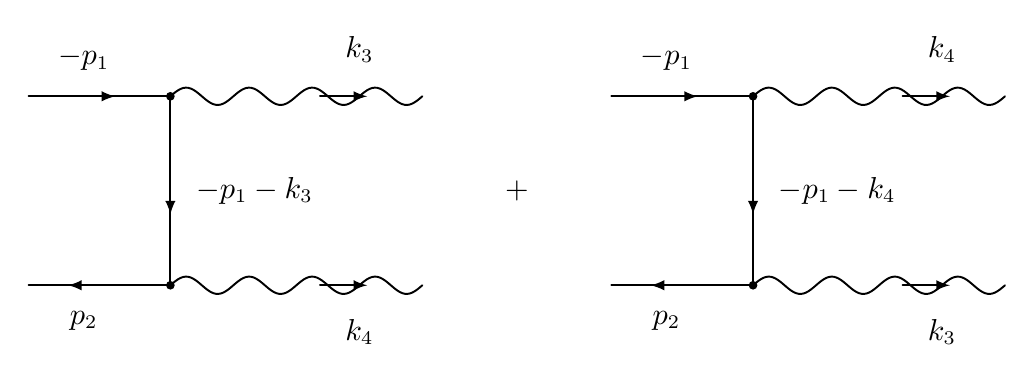
\begin{tikzpicture}[x=1mm,y=1mm,line width=.7pt,>=latex,
 line cap=round,line join=round,font=\fontsize{10.5}{12}\selectfont]
 \foreach \offset in {0,74}{
  \begin{scope}[shift={(\offset,0)}]
   \draw (0,12)--(18,12)--(18,-12)--(0,-12);
   \draw[->] (5,12)--(11,12);
   \draw[->] (18,5)--(18,-3);
   \draw[->] (11,-12)--(5,-12);
   \foreach \height in {12,-12}{
    \draw[domain=0:32,samples=101,smooth,variable=\u]
     plot ({18+\u},{\height+1.1*sin(45*\u)});
    \draw[->] (37,\height)--(43,\height);
    \fill (18,\height) circle[radius=.55mm];
   }
   \node[above] at (7,14) {$-p_1$};
   \node[below] at (7,-14) {$p_2$};
  \end{scope}
 }
 \node[right] at (20,0) {$-p_1-k_3$};
 \node[above] at (42,15) {$k_3$};
 \node[below] at (42,-15) {$k_4$};
 \node at (62,0) {$+$};
 \node[right] at (94,0) {$-p_1-k_4$};
 \node[above] at (116,15) {$k_4$};
 \node[below] at (116,-15) {$k_3$};
\end{tikzpicture}
